\section{Finding 9 - Webserver allows vulnerable Protocols}
%center under chapter title a one row table with 6 coloumns and no borders
\vspace*{-0,3cm}
\begin{center}
    \begin{tabular}{c c c c}
        \textbf{Classification:} & Misconfiguration & \textbf{Severity:} & \textbf{\textcolor{red}{High}}  
        \end{tabular}
\end{center}

The Webserver running on port 443 of the \ac{DUT} has ssl2, ssl3 and tls1 enabled. This allows accessing the Webserver with outaded protocols which are vulnerable to attacks.

\subsection{Finding Impact}
FEHLT NOCH

\subsection{Finding Details}
This is the proof for the possible usage of SSlv2 to connect to the Webserver:
\begin{figure}[h]
    \centering
    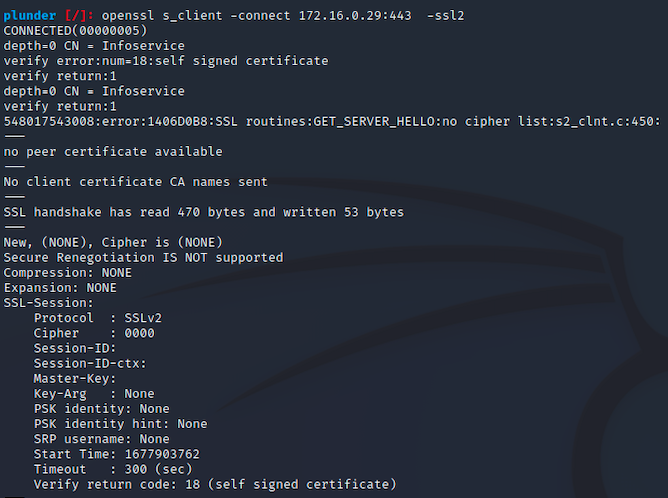
\includegraphics[width=0.8\textwidth]{img/ssl2-support.png}
    \caption{Screenshot of the Webserver}
    \label{fig:fin9}
\end{figure}

\subsection{Evaluation of Results}
\begin{center}
    \begin{tabular}{cccc}
    \textbf{Effort to Fix:} & &\ \textbf{\textcolor{orange}{Medium}}\
    \end{tabular}
\end{center}
Disable the usage of ssl2, ssl3 and tls1. This should prevent the usage of outdated protocols which are vulnerable to attacks.